\documentclass[12pt, a4paper]{article}
\usepackage[utf8]{inputenc}
\usepackage[margin=20mm]{geometry}

\usepackage{lmodern}

\usepackage{hyperref}
\hypersetup{
    colorlinks=true, % make the links colored
    linkcolor=black, % color TOC links in blue
    linktoc=all % 'all' will create links for everything in the TOC
}

\usepackage[inter-unit-product =\cdot]{siunitx}

\usepackage{amsmath}
\usepackage{amsfonts}

\usepackage[usenames, dvipsnames]{xcolor}

\usepackage{tcolorbox}

\usepackage{pgfplots}
\pgfplotsset{compat=1.9}

\usepackage{tikz}
\usetikzlibrary{arrows}
\tikzset{vecteur/.style={->, very thick, >=stealth}}
\tikzset{point/.style={color=darkgray}}
\tikzset{festat/.style={color=Green}}
\tikzset{unitaire/.style={color=violet}}
\tikzset{cestat/.style={color=blue}}

\usepackage[tikz]{bclogo}


\newcommand{\myparagraph}[1]{\paragraph{#1}\mbox{}\\}
\newcommand*\mean[1]{\overline{#1}}

\title{\textbf{Séries de Fourier}}
\author{\textit{Robin SHAMSNEJAD, cours de François BLANCHET (Polytech E2I)}}
\date{}

\begin{document}

\maketitle

\tableofcontents
\clearpage

\section{Rappels}

\subsection{Fonctions paires et impaires}

\subsubsection{Définition}

\begin{tcolorbox}
	Une fonction $f:\mathbb{R} \to \mathbb{R}$ est :
	\begin{itemize}
		\item Paire si $\forall x \in \mathbb{R}, f(-x) = f(x)$
		\item Impaire si $\forall x \in \mathbb{R}, f(-x) = -f(x)$
	\end{itemize}
\end{tcolorbox}

\subsubsection{Opérations sur les fonctions paires et impaires}

Soient $P$ une fonction paire et $I$ une fonction impaire quelconques :

\begin{itemize}
	\item Somme
		\begin{itemize}
			\item[$\cdot$] $P + I$ n'est généralement ni paire ni impaire, il faut vérifier au cas par cas
			\item[$\cdot$] $P + P$ est paire
			\item[$\cdot$] $I + I$ est impaire
		\end{itemize}
	\item Produit, on suit ce qui s'apparenterait à une sorte de << règle des signes >> :
		\begin{itemize}
			\item[$\cdot$] $P \cdot I$ est impaire
			\item[$\cdot$] $P \cdot P$ est paire
			\item[$\cdot$] $I \cdot I$ est paire
		\end{itemize}
	\item Composition
		\begin{itemize}
			\item[$\cdot$] $f \circ P$ est paire, pour n'importe quelle fonction $f$
			\item[$\cdot$] $g \circ I$ a la parité de $g$, si la fonction $g$ en a une.
		\end{itemize}
	\item Dérivation
		\begin{itemize}
			\item[$\cdot$] $P'$ est impaire
			\item[$\cdot$] $I'$ est paire
		\end{itemize}
\end{itemize}

\subsubsection{Intégration de fonctions paires et impaires}

En utilisant les propriétés de symétrie des fonctions paires et impaires, on peut utiliser les << astuces >> suivantes lorsqu'on les intègre sur un intervalle centré sur 0 :

\begin{tcolorbox}
	Soient $f:\mathbb{R} \to \mathbb{R}$ et $a \in \mathbb{R}$ :
	\begin{itemize}
		\item Si $f$ est paire, $\displaystyle \int_{-a}^{a} f(t)dt = 2 \int_0^{a} f(t)dt = 2 \int_{-a}^{0} f(t)dt$
		\item Si $f$ est impaire, $\displaystyle \int_{-a}^{a} f(t)dt = 0$
	\end{itemize}
\end{tcolorbox}

\subsection{Fonctions périodiques}

La fonction sinus est un exemple de fonction périodique :

	\begin{center}
	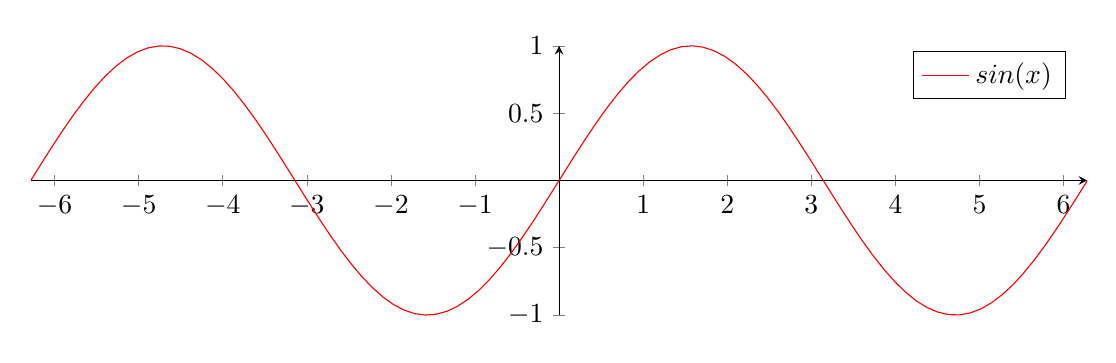
\begin{tikzpicture}
		\begin{axis}[axis lines=middle, height=5cm, width=15cm]
			\addplot[domain=-2*pi:2*pi, samples=100, color=red] {sin(deg(x))};
			\addlegendentry{$sin(x)$}
		\end{axis}
	\end{tikzpicture}
	\end{center}
	
\begin{tcolorbox}
	Une fonction $f:\mathbb{R} \to \mathbb{R}$ est périodique de période T si :
	\begin{equation*}
		\forall t \in \mathbb{R}, f(t + T) = f(t)
	\end{equation*}
\end{tcolorbox}

\subsection{Fonctions continues par morceaux}

La fonction suivante est un exemple de fonction continue par morceaux :

	\begin{equation*}
		\forall x \in \mathbb{R}, f(x) = (-1)^{\lfloor x \rfloor}
	\end{equation*}
	
	\begin{center}
	\begin{tikzpicture}
		\begin{axis}[axis lines=middle, height=5cm, width=15cm]
			%\addplot[domain=-2:2, samples=1000, color=red] {(-1)^floor(x)};
			\addplot[domain=-2:2, samples=100, color=red] coordinates {(-2,1) (-1,1)};
			\addplot[domain=-2:2, samples=100, color=red] coordinates {(-1,-1) (0,-1)};
			\addplot[domain=-2:2, samples=100, color=red] coordinates {(0,1) (1,1)};
			\addplot[domain=-2:2, samples=100, color=red] coordinates {(1,-1) (2,-1)};
			\addlegendentry{$(-1)^{\lfloor x \rfloor}$}
		\end{axis}
	\end{tikzpicture}
	\end{center}

\begin{tcolorbox}
	\underline{Définition simplifiée} : Une fonction continue par morceaux est une fonction qui, en chaque réel où elle << saute >>, a une limite finie de chaque côté.
\end{tcolorbox}

Si on prend par exemple le saut en $x = 1$, on a : $\displaystyle\lim_{x \to 1^-} f(x) = 1$ et $\displaystyle\lim_{x \to 1^+} f(x) = -1$. On notera ces limites respectivement $f(1^-)$ et $f(1^+)$.

Pour dire que la fonction f est continue par morceaux, on dit qu'elle appartient à un ensemble noté $C_{pm}^0$ ou $C_{mcx}^0$ (il n'y a pas vraiment de notation internationale officielle). Ce qui donnera la notation suivante :

\begin{tcolorbox}
	Si f est continue par morceaux, définie sur $[a,b]$ et à valeurs dans $\mathbb{R}$,  on note :
		
		\begin{equation*}
			f \in C_{pm}^0([a,b] \to \mathbb{R})
		\end{equation*}
\end{tcolorbox}



\clearpage



On considérera notamment des fonctions à valeurs complexes du type :

	\begin{align*}
		\begin{cases}
			f:\mathbb{R} \to \mathbb{C} \\
			a \in C_{pm}^0(\mathbb{R} \to \mathbb{R}) \\
			b \in C_{pm}^0(\mathbb{R} \to \mathbb{R})
		\end{cases} \\
		f(t) = a(t) + i \cdot b(t) \Rightarrow f \in C_{pm}^0(\mathbb{R} \to \mathbb{C})
	\end{align*}

On saura les intégrer : $\displaystyle\int f(t)dt = \int a(t)dt + i \cdot \int b(t)dt $ 

Par exemple :

	\begin{equation*}
		\begin{aligned}
			\int e^{i\alpha t} dt & = \int (cos(\alpha t) + i \cdot sin(\alpha t))dt \\
			{} & = \int cos(\alpha t) dt + i \cdot \int sin(\alpha t) dt \\
			{} & = \frac{1}{\alpha} \cdot sin(\alpha t) - \frac{i}{\alpha} \cdot cos(\alpha t) \\
			{} & = -\frac{i}{\alpha} ( cos(\alpha t) + i \cdot sin(\alpha t) ) \\
			{} & = -\frac{i}{\alpha} e^{i \alpha t} \\
			{} & = \frac{1}{i\alpha} e^{i\alpha t}
		\end{aligned}
	\end{equation*}

On peut généraliser :

	\begin{equation*}
		\begin{aligned}
			\forall z \in \mathbb{C}, \int e^{zt} dt = \frac{1}{z} e^{zt}
		\end{aligned}
	\end{equation*}


\subsection{Combinaison}

\begin{tcolorbox}
	Si $f:\mathbb{R} \to \mathbb{C}$ est T-périodique et continue par morceaux, on note :
	\begin{equation*}
		f \in C_{pm}^0(T, \mathbb{R} \to \mathbb{C})
	\end{equation*}
\end{tcolorbox}





\clearpage





\section{Coefficients et série de Fourier}

La série de Fourier est un outil mathématique permettant la décomposition d'un signal périodique en un ensemble de sinusoïdes, qui, une fois recombinées, permettent d'obtenir une approximation de ce signal. C'est un outil fondamental pour des domaines tels que l'analyse harmonique et le traitement du signal.

\subsection{Coefficients de Fourier}
\subsubsection{Définition}

\begin{tcolorbox}
	Pour une fonction $f \in C_{pm}^0(T, \mathbb{R} \to \mathbb{C})$, on définit avec $\displaystyle\omega = \frac{2\pi}{T}$ :
	\begin{itemize}
		\item Les coefficients de Fourier complexes
			\begin{equation*}
				\forall n \in \mathbb{Z}, ~ C_n(f) = \frac{1}{T} \int_T [f(t)e^{-in\omega t}]dt
			\end{equation*}
		\item Les coefficients de Fourier réels
			\begin{equation*}
				\forall n \in \mathbb{N}, ~ 
				\begin{cases}
					\displaystyle
					a_n(f) = \frac{2}{T} \int_T [f(t) cos(n\omega t)]dt \\
					{} \\
					\displaystyle
					b_n(f) = \frac{2}{T} \int_T [f(t) sin(n\omega t)]dt
				\end{cases}
			\end{equation*}
	\end{itemize}
\end{tcolorbox}

\myparagraph{Remarque}

La notation $\displaystyle\int_T$ signifie que l'on intègre une fonction T-périodique sur un intervalle quelconque, \textbf{pourvu qu'il soit de taille $T$} (sa période, donc). Cela sous-entend que l'intégrale ne dépend pas de l'intervalle choisi.

\subsubsection{Remarques}

\begin{itemize}
	\item $\displaystyle C_0(f) = \frac{a_0(f)}{2}$ est la valeur moyenne de $f$ sur $T$ :
		\begin{align*}
			\begin{cases}
				\displaystyle
				C_0(f) = \frac{1}{T} \int_T [f(t)e^{0}]dt \\
				\displaystyle
				a_0(f) = \frac{2}{T} \int_T [f(t) cos(0)]dt
			\end{cases} \\
			\Rightarrow C_0(f) = \frac{a_0(f)}{2} = \frac{1}{T} \int_T f(t)dt
		\end{align*}
	\item Si $f = cos$, alors $a_1(f) = 1$ et tous les autres $a_n(f)$ et $b_n(f)$ sont nuls
	\item $a_n(f)$ et $b_n(f)$ \textbf{ n'ont pas toujours une valeur réelle }. Exemple :
		\begin{align*}
			f(t) = e^{i\omega t} = cos(\omega t) + i \cdot sin(\omega t) \\
			\begin{cases}
				a_1(f) = 1 \\
				b_1(f) = i \\
				\forall n \in \mathbb{N}\setminus \{1\}, a_n(f) = b_n(f) = 0
			\end{cases}
		\end{align*}
\end{itemize}

\subsubsection{Cas de la parité}

\begin{tcolorbox}
	Si $f \in C_{pm}^0(T, \mathbb{R} \to \mathbb{C})$ est :
	\begin{itemize}
		\item Paire :
			\begin{equation*}
				\forall n \in \mathbb{N},
					\begin{cases}
						\displaystyle
						a_n(f) = \frac{2}{T} \int_T [f(t) cos(n\omega t)]dt = \frac{4}{T} \int_0^{\frac{T}{2}} [f(t) cos(n\omega t)]dt \\
						{} \\
						\displaystyle
						b_n(f) = 0
					\end{cases}
			\end{equation*}
		\item Impaire :
			\begin{equation*}
				\forall n \in \mathbb{N}, ~ 
				\begin{cases}
					\displaystyle
					a_n(f) = 0 \\
					{} \\
					\displaystyle
					b_n(f) = \frac{2}{T} \int_T [f(t) sin(n\omega t)]dt = \frac{4}{T} \int_0^{\frac{T}{2}} [f(t) sin(n\omega t)]dt
				\end{cases}
			\end{equation*}
	\end{itemize}
\end{tcolorbox}

\subsection{Analyse d'une fonction par série de Fourier}

\subsubsection{Somme partielle de la série de Fourier}

La somme partielle d'indice $N$ de la série de Fourier de la fonction $f \in C_{pm}^0(T, \mathbb{R} \to \mathbb{C})$ est définie comme :

\begin{itemize}
	\item Avec les coefficients complexes :
		\begin{itemize}
			\item[$\cdot$]
				$\displaystyle SF_0(f) = C_0(f)$
			\item[$\cdot$]
				$\displaystyle \forall N \in \mathbb{N}^{*}, ~ SF_N(f(t)) = C_0(f) + \sum_{n = 1}^{N}[C_n(f)e^{in\omega t} + C_{-n}(f)e^{-in\omega t}]$
		\end{itemize}

	\item Avec les coefficients réels :
		\begin{itemize}
			\item[$\cdot$]
				$\displaystyle SF_0(f) = \frac{a_0(f)}{2}$
			\item[$\cdot$]
				$\displaystyle \forall N \in \mathbb{N}^{*}, ~ SF_N(f(t)) = \frac{a_0(f)}{2} + \sum_{n = 1}^{N}[a_n(f)cos(n\omega t) + b_n(f)sin(n\omega t)]$
		\end{itemize}
\end{itemize}

\subsubsection{Série de Fourier d'une fonction}

\begin{tcolorbox}
	Soit $f \in C_{pm}^0(T, \mathbb{R} \to \mathbb{C})$
	
	On appelle la \textbf{série de Fourier} de $f$ :
	
	\begin{equation*}
		SF(f) = \lim_{n\to\infty} SF_n(f)
	\end{equation*}
	\begin{itemize}
		\item Avec les coefficients complexes :
			\begin{equation*}
				\begin{aligned}
					SF(f)(t) & = \sum_{n = -\infty}^{+\infty}[C_n(f)e^{in\omega t}] \\
					SF(f)(t) & = C_0(f) + \sum_{n = 1}^{+\infty}[C_n(f)e^{in\omega t} + C_{-n}(f)e^{-in\omega t}] \\
				\end{aligned}
			\end{equation*}

		\item Avec les coefficients réels :
			\begin{equation*}
				SF(f)(t) = \frac{a_0(f)}{2} + \sum_{n = 1}^{+\infty}[a_n(f)cos(n\omega t) + b_n(f)sin(n\omega t)]
			\end{equation*}
	\end{itemize}
	Avec $\displaystyle\omega = \frac{2\pi}{T}$
\end{tcolorbox}

\subsubsection{Interprétation physique}

La \textbf{suite de fonctions} à laquelle est associée la série de Fourier est :

\begin{itemize}
	\item Avec les coefficients complexes :
		\begin{itemize}
			\item[$\cdot$]
				$\displaystyle U_0(f) = C_0(f)$
			\item[$\cdot$]
				$\displaystyle \forall n \in \mathbb{N}^{*}, ~ U_n(f)(t) = C_n(f)e^{in\omega t} + C_{-n}(f)e^{-in\omega t}$
		\end{itemize}

	\item Avec les coefficients réels :
		\begin{itemize}
			\item[$\cdot$]
				$\displaystyle U_0(f) = \frac{a_0(f)}{2}$
			\item[$\cdot$]
				$\displaystyle \forall n \in \mathbb{N}^{*}, ~ U_n(f)(t) = a_n(f)cos(n\omega t) + b_n(f)sin(n\omega t)$
		\end{itemize}
\end{itemize}

Cette suite est appelée le \textbf{spectre} de $f$, et un terme de rang $n$ de cette suite est appelé \textbf{harmonique de rang $n$}. Plus particulièrement, l'harmonique de rang 0 est une constante et sera généralement appelée la \textbf{composante continue}, et l'harmonique de rang 1 est appelée la \textbf{fondamentale}.

La série de Fourier nous apprend donc que toute fonction périodique de pulsation $\displaystyle \omega = \frac{2\pi}{T}$ est décomposable en une somme d'harmoniques, qui sont des fonctions sinusoïdales.

\begin{tcolorbox}
	ATTENTION : une fonction n'est pas nécessairement égale à sa série de Fourier sur tout son domaine de définition $\rightarrow$ voir le théorème de Dirichlet
\end{tcolorbox}

Chaque harmonique de rang $n$ a une pulsation qui vaut $n\omega$, et donc une période qui vaut :
\begin{equation*}
	T_n = \frac{2\pi}{n\omega} = \frac{T}{n}
\end{equation*}



\clearpage




\section{Théorème de Parseval}

\subsection{Définition}

\begin{tcolorbox}
	L'intégrale de Parseval de $f \in C_{pm}^0(T, \mathbb{R} \to \mathbb{C})$ est définie par :
	
	\begin{itemize}
		\item Avec les coefficients complexes :
			\begin{equation*}
				\frac{1}{T} \int_T |f(t)|^2 dt = \sum_{n=-\infty}^{+\infty} |C_n(f)|^2
			\end{equation*}
		\item Avec les coefficients réels :
			\begin{equation*}
				\frac{1}{T} \int_T |f(t)|^2 dt = \left|\frac{a_0(f)}{2}\right|^2 + \sum_{n=1}^{+\infty} \left( \frac{1}{2}|a_n(f)|^2 + \frac{1}{2}|b_n(f)|^2 \right)
			\end{equation*}
	\end{itemize}

	\textbf{Attention} : ici, $|~|$ désigne bien un module complexe.
\end{tcolorbox}

\subsection{Cas de la parité}

Soit $f \in C_{pm}^0(T, \mathbb{R} \to \mathbb{C})$. Si $f$ est paire ou impaire, alors son intégrale de Parseval peut s'écrire sur une demi-période et peut s'écrire :

	\begin{itemize}
		\item Si f est paire :
			\begin{equation*}
				\frac{2}{T} \int_0^{\frac{T}{2}} |f(t)|^2 dt = \left|\frac{a_0(f)}{2}\right|^2 + \sum_{n=1}^{+\infty} \left( \frac{1}{2}|a_n(f)|^2 \right)
			\end{equation*}
		\item Si f est impaire :
			\begin{equation*}
				\frac{2}{T} \int_0^{\frac{T}{2}} |f(t)|^2 dt = \sum_{n=1}^{+\infty} \left( \frac{1}{2}|b_n(f)|^2 \right)
			\end{equation*}
	\end{itemize}

\subsection{Interprétation physique}

\subsubsection{Rappels}

\begin{itemize}
	\item Pour une fonction $g:\mathbb{R} \to \mathbb{C}$ quelconque, on définit sa valeur moyenne sur un intervalle $[\alpha, \beta] \subset \mathbb{R}$ comme :
		\begin{equation*}
			\mean{g}_{[\alpha, \beta]} = \frac{1}{\beta - \alpha} \int_\alpha^\beta g(t)dt
		\end{equation*}
	\item Pour une fonction $h:\mathbb{R} \to \mathbb{C}$ quelconque, on définit sa puissance instantanée en $t$ comme :
		\begin{equation*}
			P_h(t) = |h(t)|^2
		\end{equation*}
\end{itemize}

\subsubsection{Puissance moyenne}

D'après les rappels précédents :

\begin{tcolorbox}
	L'intégrale de Parseval d'une fonction $f$ périodique est égale à la puissance moyenne de $f$ sur une période
\end{tcolorbox}

\subsubsection{Décomposition de la formule}

%	\begin{equation*}
%		\colorbox{red!50}{$\displaystyle \frac{1}{T} \int_T |f(t)|^2 dt$} = \colorbox{green!50}{$\displaystyle \frac{1}{2} \left( \frac{|a_0(f)|^2}{2} \right)$} + \colorbox{blue!50}{$\displaystyle \sum_{n=1}^{+\infty} \left( \frac{1}{2}|a_n(f)|^2 + \frac{1}{2}|b_n(f)|^2 \right)$}
%	\end{equation*}

\begin{tcolorbox}
	Le théorème de Parseval nous indique ainsi que la puissance moyenne d'une fonction $f \in C_{pm}^0(T, \mathbb{R} \to \mathbb{C})$ vaut la somme de puissances moyennes de toutes ses harmoniques :

	\begin{equation*}
		\underbrace{ \frac{1}{T} \int_T |f(t)|^2 dt }_{\text{\parbox{2,5cm}{Puissance moyenne de $f$ sur $T$}}} = \underbrace{ \left|\frac{a_0(f)}{2}\right|^2}_{\text{\parbox{2,5cm}{Puissance moyenne de l'harmonique de rang $0$ sur $T$}}} + \sum_{n=1}^{+\infty} \underbrace{\left( \frac{1}{2}|a_n(f)|^2 + \frac{1}{2}|b_n(f)|^2 \right)}_{\text{\parbox{3cm}{Puissance moyenne de l'harmonique de rang $n$ sur $T$}}}
	\end{equation*}
\end{tcolorbox}

\section{Théorème de Dirichlet}

\subsection{Introduction}

Pour ce théorème, on considère des fonctions continues par morceaux, et dont les dérivées sont également continues par morceaux :

\begin{tcolorbox}
	Si $f \in C_{pm}^0(\mathbb{R} \to \mathbb{C})$ et $f' \in C_{pm}^0(\mathbb{R} \to \mathbb{C})$, alors on note $f \in C_{pm}^1(\mathbb{R} \to \mathbb{C})$
\end{tcolorbox}

\subsection{Énoncé}

\begin{tcolorbox}
	Si $f \in C_{pm}^1(T,\mathbb{R} \to \mathbb{C})$, alors :
	
	\begin{equation*}
		\forall t \in \mathbb{R}, SF(f)(t) = \frac{1}{2}\left(f(t^-) + f(t^+)\right)
	\end{equation*}

	En particulier, si $f$ est continue sur tout $\mathbb{R}$, alors :
	
	\begin{equation*}
		\forall t \in \mathbb{R}, ~ f(t^-) = f(t^+) = f(t)
	\end{equation*}
	
	Dans ce cas, le théorème de Dirichlet peut s'écrire :
	\begin{equation*}
		\forall t \in \mathbb{R}, ~ SF(f)(t) = f(t)
	\end{equation*}
\end{tcolorbox}

En d'autres termes : une fonction est égale à sa série de Fourier sur tout son domaine de définition seulement si elle est continue. Si elle est continue par morceaux, c'est également vrai << à peu près partout >>, sauf aux points de discontinuité où sa série de Fourier est égale à la moyenne de ses limites de chaque côté.



\clearpage



\section{Intégration et dérivation d'une série de Fourier}

\subsection{Intégration}

On admet qu'on peut intégrer une série terme à terme. Ainsi :

\begin{tcolorbox}
	Si $f \in C_{pm}^1$ et $f \in C^0$, alors on peut intégrer $SF(f)$ terme à terme :
	\begin{equation*}
		\begin{aligned}
			\int SF(f) & = \int\left(\frac{a_0(f)}{2}\right) + \sum_{n = 1}^{+\infty}\left(\int\left[a_n(f)cos(n\omega t) + b_n(f)sin(n\omega t)\right]\right)
		\end{aligned}
	\end{equation*}
\end{tcolorbox}

\subsection{Dérivation}

\begin{tcolorbox}
	Si $f \in C_{pm}^1$ et $f \in C^0$, alors on peut obtenir $SF(f')$ en dérivant $SF(f)$ terme à terme :
	\begin{equation*}
		SF(f') = \frac{d}{dt}\left(\frac{a_0(f)}{2}\right) + \sum_{n = 1}^{+\infty}\left(\frac{d}{dt}\left[a_n(f)cos(n\omega t) + b_n(f)sin(n\omega t)\right]\right)
	\end{equation*}
\end{tcolorbox}

\subsection{Remarque}

Ces propriétés sont surtout utiles dans le cas où on peut utiliser le théorème de Dirichlet : dans ce cas, l'intégrale terme à terme de la série de Fourier d'une fonction $f$ vaut l'intégrale de $f$ ; et il en va de même pour la dérivation.


\end{document}
